% Teil: Mengen-Funktionen-Relationen
% Kapitel: Relationen
% Abschnitt: Graphen

\documentclass[../../../include/open-logic-section]{subfiles}

\begin{document}

\olfileid{sfr}{rel}{grp}
\olsection{Graphen}

Ein \emph{Graph} ist ein Diagramm, in dem Punkte - sogenannte \glqq Knoten\grqq{} oder
\glqq Ecken\grqq{} durch Kanten verbunden sind.  Graphen
sind ein allgegenwärtiges Werkzeug in der diskreten Mathematik und in der Informatik.
Sie sind außerordentlich nützlich, um Beziehungen und Strukturen darzustellen,
von konkreten Dingen wie verschiedenen Netzwerken bis hin zu abstrakten Strukturen wie den möglichen Ergebnissen in
Entscheidungssituationen.  In der Literatur gibt es viele verschiedene Arten von Graphen,
die sich z. B. darin unterscheiden, ob die Kanten gerichtet oder ungerichtet sind,
ob sie beschriftet sind, ob es Kanten von einem Knoten zum
gleichen Knoten gebe nkann, oder mehrere Kanten zwischen den gleichen Knoten, etc.
\emph{Gerichtete Graphen} haben eine besondere Beziehung zu Relationen.

\begin{defn}[Gerichteter Graph]
Ein \emph{gerichteter Graph} $G = \tuple{V, E}$ ist eine Menge von
\emph{Knoten}~$V$ und eine Menge von \emph{Kanten}~$E \subseteq V^2$.
\end{defn}

\begin{explain}
Nach unserer Definition ist ein Graph einfach eine Menge zusammen mit einer
Relation auf dieser Menge.  Wenn man über Graphen spricht, ist es nur
natürlich, dass sie grafisch dargestellt werden: Wir können einen
Graphen zeichnen, indem wir zwei Knoten~$v_1$ und $v_2$ durch einen Pfeil verbinden
gdw $\tuple{v_1, v_2} \in E$.  Der einzige Unterschied zwischen einer Relation an sich
und einem Graphen besteht darin, dass ein Graph die Menge der Knoten angibt,
d. h., ein Graph kann isolierte Knoten haben. Der wichtige Punkt
ist jedoch, dass jede Relation~$R$ auf einer Menge~$X$ als ein
gerichteter Graph $\tuple{X, R}$ betrachtet werden kann, und umgekehrt ein gerichteter
Graph~$\tuple{V, E}$ als eine Relation $E \subseteq V^2$ angesehen werden kann, wobei
die Menge $V$ explizit angegeben ist.
\end{explain}

\begin{ex}
Der Graph $\tuple{V, E}$ mit $V = \{1, 2, 3, 4\}$ und $E =
\{\tuple{1,1}, \allowbreak \tuple{1, 2}, \allowbreak \tuple{1, 3},
\allowbreak \tuple{2, 3}\}$ sieht wie folgt aus:
\begin{align*}
& 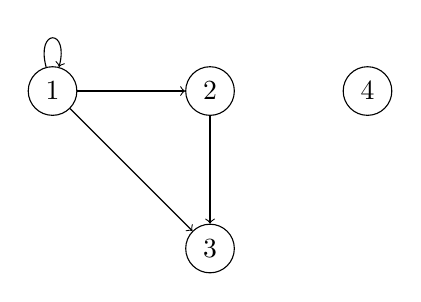
\begin{tikzpicture}[->,node distance=2cm]
  \node[draw,circle] (A) {$1$};
  \node[draw,circle] (B) [right of=A] {$2$};
  \node[draw,circle] (C) [below of=B] {$3$};
  \node[draw,circle] (D) [right of=B] {$4$};
  \draw (A) to [loop above] (A);
  \draw (A) to (B);
  \draw (A) to (C);
  \draw (B) to (C);
  \end{tikzpicture}
\intertext{Dies ist ein anderer Graph als $\tuple{V', E}$ mit $V' =
  \{1, 2, 3\}$, der wie folgt aussieht:}
  & 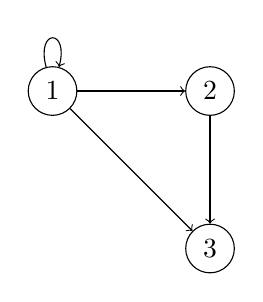
\begin{tikzpicture}[->,node distance=2cm]
    \node[draw,circle] (A) {$1$};
    \node[draw,circle] (B) [right of=A] {$2$};
    \node[draw,circle] (C) [below of=B] {$3$};
    \draw (A) to [loop above]  (A);
    \draw (A) to  (B);
    \draw (A) to  (C);
    \draw (B) to  (C);
  \end{tikzpicture}
\end{align*}
\end{ex}

\begin{prob}
  Betrachten Sie die kleiner-gleich-Relation~$\le$ auf der Menge $\{1,
  2, 3, 4\}$ als Graph und zeichnen Sie das entsprechende Diagramm.
\end{prob}

\end{document}